\begin{figure}[tb]
\centering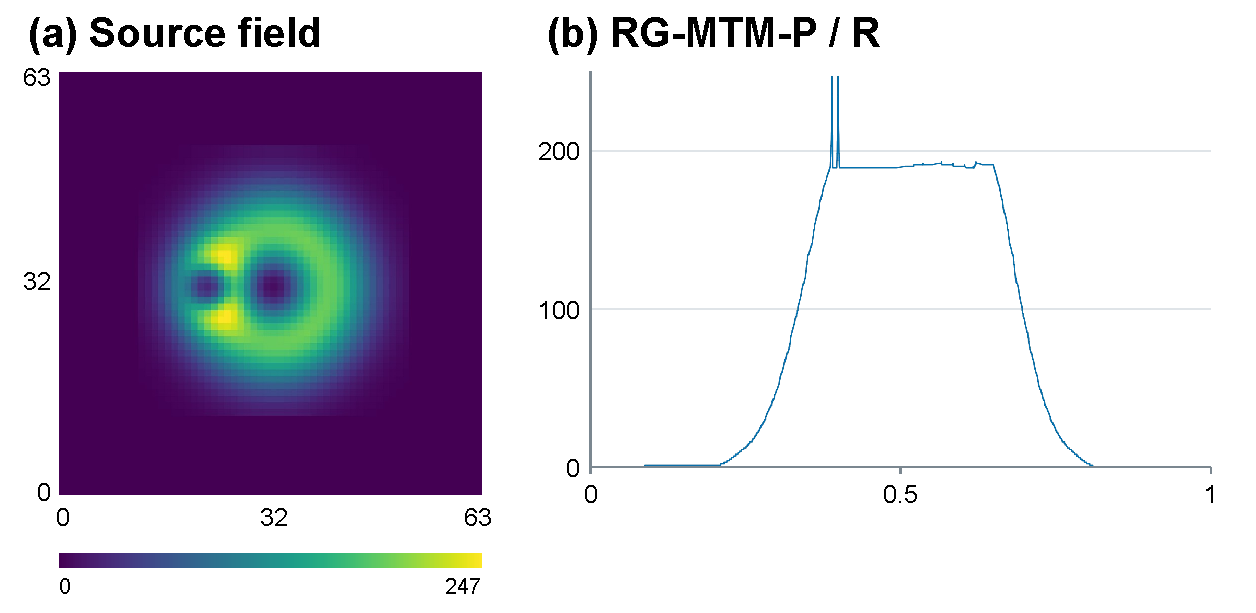
\includegraphics[width=\linewidth]{figures/Fig8.pdf}
\caption{Nucleon: the unchanged author $64\times64$ scalar slice (a) and the complete RG-MTM-P profile (b, 32768 samples). Every R setting returns exactly the same profile as P. Both panels retain the original scalar units. NROE is 2.38\%, with zero measured NMLE. This is one static slice; the TMTM comparison is in Supplement S10.}
\label{fig:nucleon}
\end{figure}

\begin{figure*}[t]
\centering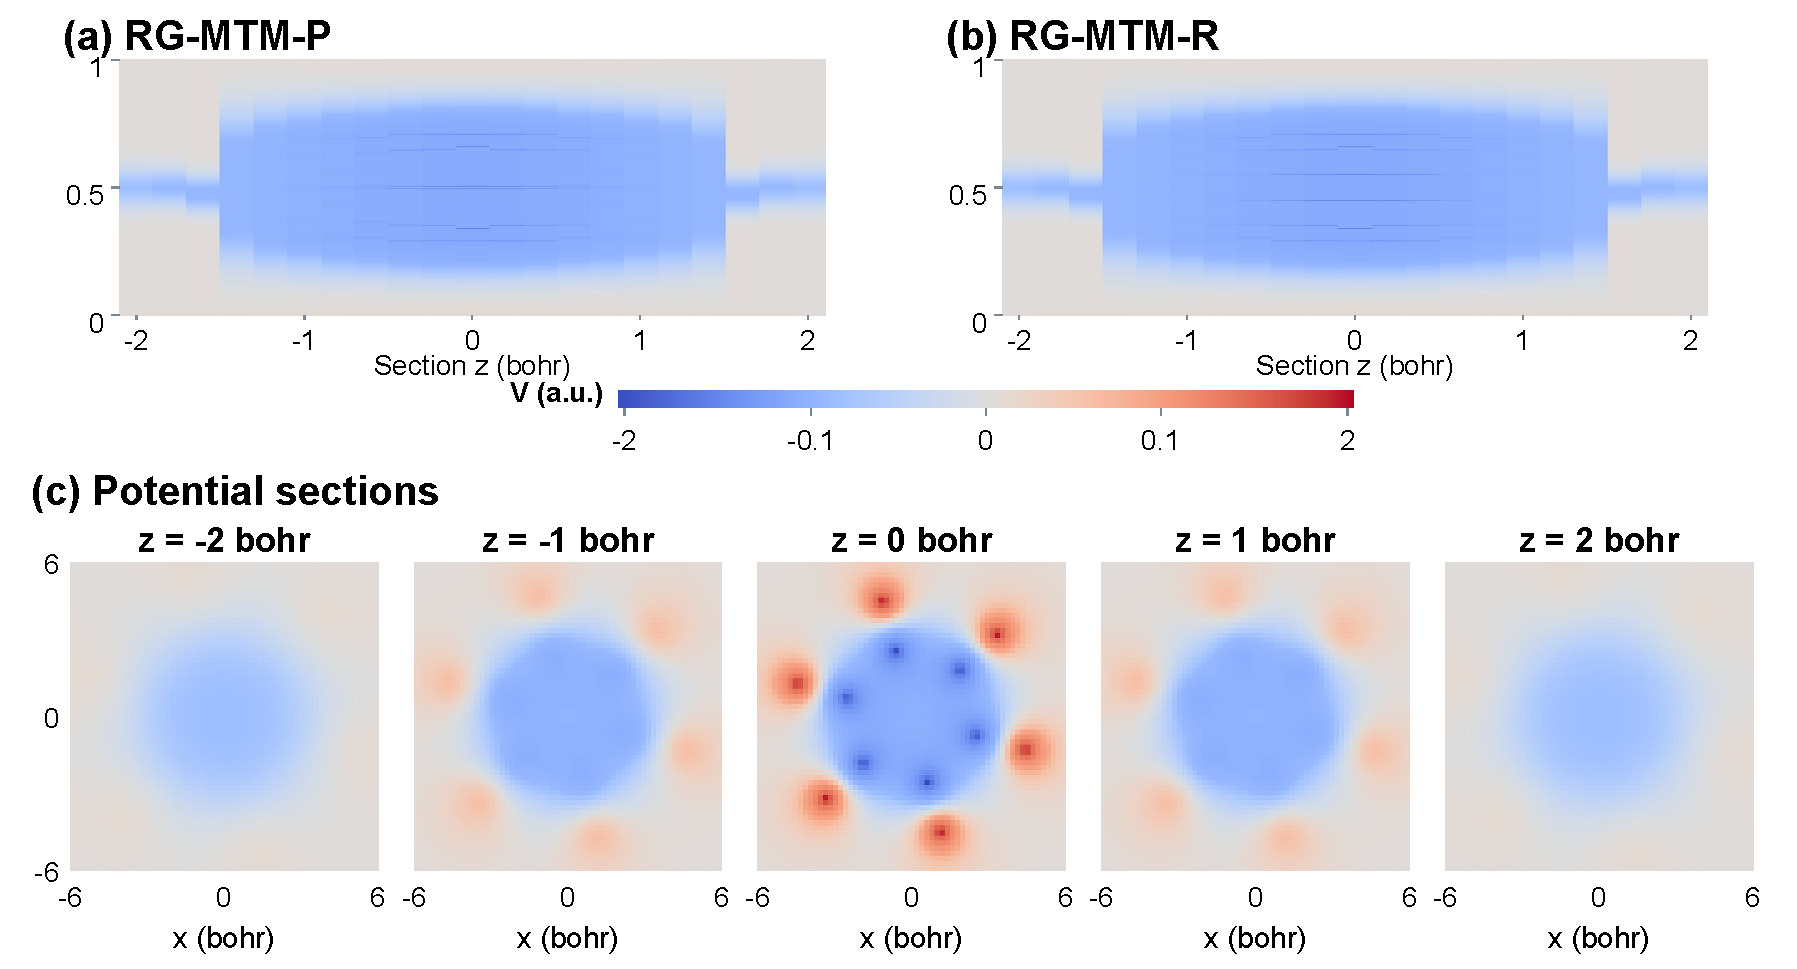
\includegraphics[width=\textwidth]{figures/Fig9.pdf}
\caption{Benzene: RG-MTM-P/R2 maps of all 21 static $z$ sections (a,b), with source potential at $z=-2,-1,0,1,2$ bohr (c). Section $z$ is a spatial coordinate. Maps and source fields share a symmetric-log scale, linear within $\pm0.0784$ a.u.; potential is in Hartree/$e$. This is the declared OPLS-AA reconstruction. The TMTM comparison is in Supplement S10; full and interior-extremum scores are in S9.}
\label{fig:benzene}
\end{figure*}

\subsubsection{Nucleon: Static Scalar Structure}\label{sec:nucleon}
Nucleon tests a static layout on the TMTM authors' original padded $64\times64$ scalar slice~\cite{Koepp:2023:TMTM}. Figure~\ref{fig:nucleon} pairs the complete source slice (a) with the complete P/R scalar profile (b). Both panels describe the same static input. The input has one frame and 13 extracted extrema; the derived tree has 26 nodes, compared with 28 in the reference table. The source samples are unchanged, and no simplification threshold is applied. TMTM has 11.90\% NROE, while P has 2.38\%; both have zero measured NMLE. Table~\ref{tab:tradeoff} group its order, merge-level, and displacement measurements with the other planar inputs. All three R settings return exactly the same saved profile as P, so relaxation adds no benefit in this case. This null relaxation result shows that reference guidance can improve a legal order without requiring a scalar trade-off. The added ST-MTM run has 11.90\% NROE and zero NMLE; its stronger SNS/TW (Table~\ref{tab:tradeoff}) shows that this static reference-order gain does not imply a relative-geometry gain. The example supplies a static scalar comparison; its single slice supports neither temporal nor volumetric claims.

\subsubsection{Benzene: Reconstructed Electrostatic Potential}\label{sec:benzene}
The Benzene experiment uses an explicitly reconstructed electrostatic potential, rather than the unavailable original author file. An OPLS-AA point-charge model assigns $-0.115e$ to each carbon and $+0.115e$ to each hydrogen~\cite{Jorgensen:2013:BOSS}. Atomic positions come from the header of a public Inviwo molecular cube~\cite{Inviwo:BenzeneGeometry}; its electron-density samples are not used. We evaluate $V(r)=\sum_iq_i/\|r-R_i\|$ on 21 parallel $61\times61$ sections, with $x,y\in[-6,6]$ and $z\in[-2,2]$ in bohr. Section $z$ is a spatial coordinate of a static field, not physical time. This classical reconstruction is a model-specific comparison, not the original fractional-charge potential or a quantum-chemical reproduction.

Figure~\ref{fig:benzene} pairs the P/R slice maps with five source sections; Supplement S10 retains the full baseline comparison. Join trees retain low-potential extrema after a common 0.05\% per-section persistence simplification. P reduces mean NROE from 50.00\% to 4.21\% while preserving merge levels. Each R setting reaches zero NROE with 0.0025\% mean and 0.0080\% maximum NMLE; the three settings have identical measured results. The added ST-MTM run also has 50.00\% mean NROE and zero NMLE, with lower SNS than P/R but larger adjacent-section displacement than R. Neither TMTM nor ST-MTM optimizes the supplied $x$ reference, so these values assess reference compatibility rather than its original objective.

Four boundary extrema occur in every section and contribute substantially to the complete-leaf score. On the 15 sections with at least two interior extrema, interior-only NROE is 12.50\% for TMTM, 5.89\% for P, and zero for R. Across 170 overlap matches, mean adjacent-section displacement residual is 2.755\% for TMTM, 1.219\% for P, and 0.137\% for R. Mean $\pm z$ map discrepancy similarly changes from 0.0185\% to 0.0064\% to 0.0030\%. The source field is only approximately mirror-symmetric: its maximum paired discrepancy is 0.0241\% of scalar range. These are slice-coherence diagnostics, not molecular-motion errors (Supplement S9). Keeping the boundary and full-population results together makes the scope of the apparent position gain explicit.
